\documentclass{article}
\usepackage[utf8]{inputenc}
\usepackage{pgfplots}
\usepackage{pgfplotstable}
\usepackage{booktabs}
\usepackage{geometry}
\usepackage{float}
\usepackage{xcolor}
\usepackage{pagecolor}

% Define custom colors with better contrast
\definecolor{concrete}{RGB}{100,100,100}
\definecolor{bricks}{RGB}{200,50,50}
\definecolor{aac}{RGB}{50,150,200}
\definecolor{asphalt}{RGB}{30,30,30}
\definecolor{freespace}{RGB}{240,240,240}
\definecolor{pagebg}{RGB}{242,242,242}

% Set page margins
\geometry{
    a4paper,
    margin=2.5cm
}

% Set page background color
\pagecolor{pagebg}

\begin{document}

\begin{figure}[H]
\centering
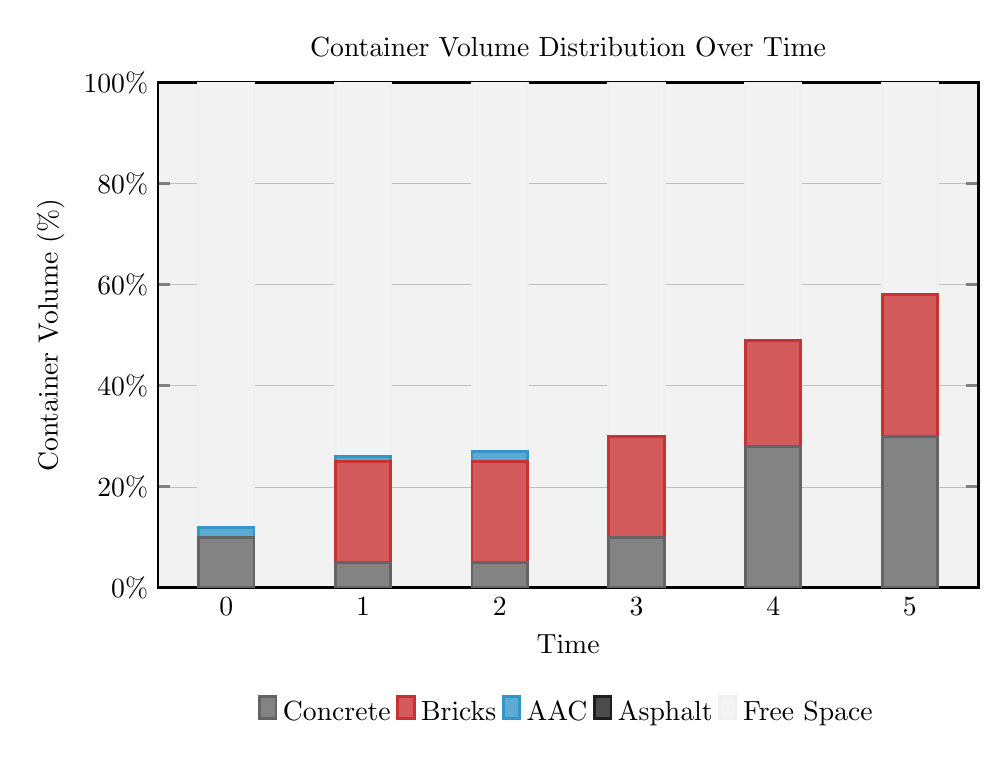
\begin{tikzpicture}
\begin{axis}[
    width=12cm,
    height=8cm,
    xlabel={Time},
    ylabel={Container Volume (\%)},
    xmin=-0.5, xmax=5.5,
    ymin=0, ymax=100,
    grid=both,
    grid style={line width=.1pt, draw=gray!10},
    major grid style={line width=.2pt,draw=gray!50},
    legend style={
        at={(0.5,-0.2)},
        anchor=north,
        legend columns=5,
        draw=none,
        fill=none
    },
    axis line style={line width=1pt},
    tick style={line width=1pt},
    title style={align=center},
    title={Container Volume Distribution Over Time},
    ytick={0,20,40,60,80,100},
    xtick={0,1,2,3,4,5},
    xticklabels={0,1,2,3,4,5},
    yticklabels={0\%,20\%,40\%,60\%,80\%,100\%},
    axis background/.style={fill=pagebg},
    stack plots=y,
    ybar stacked,
    bar width=20pt,
    every axis plot/.append style={line width=1pt}
]

% Concrete (bottom layer)
\addplot[concrete,fill=concrete!80] coordinates {
    (0,10)
    (1,5)
    (2,5)
    (3,10)
    (4,28)
    (5,30)
};

% Bricks (second layer)
\addplot[bricks,fill=bricks!80] coordinates {
    (0,0)
    (1,20)
    (2,20)
    (3,20)
    (4,21)
    (5,28)
};

% AAC (third layer)
\addplot[aac,fill=aac!80] coordinates {
    (0,2)
    (1,1)
    (2,2)
    (3,0)
    (4,0)
    (5,0)
};

% Asphalt (fourth layer)
\addplot[asphalt,fill=asphalt!80] coordinates {
    (0,0)
    (1,0)
    (2,0)
    (3,0)
    (4,0)
    (5,0)
};

% Free space (top layer)
\addplot[freespace,fill=freespace!80] coordinates {
    (0,100)
    (1,80)
    (2,75)
    (3,70)
    (4,51)
    (5,42)
};

\legend{Concrete, Bricks, AAC, Asphalt, Free Space}

\end{axis}
\end{tikzpicture}
\caption{Container volume distribution over time showing material accumulation}
\label{fig:capacity_chart}
\end{figure}

\end{document} 